\documentclass[11pt,a4paper]{article}

\usepackage[margin=1in]{geometry}
\usepackage{amsmath,amssymb}
\usepackage{graphicx}
\usepackage{float}
\usepackage{booktabs}
\usepackage{caption}
\usepackage{subcaption}
\usepackage{xcolor}
\usepackage{listings}
\usepackage[hidelinks]{hyperref}

\lstdefinestyle{matlabstyle}{
    language=Matlab,
    basicstyle=\ttfamily\small,
    keywordstyle=\color{blue!70!black},
    commentstyle=\color{green!45!black},
    stringstyle=\color{red!60!black},
    numbers=left,
    numberstyle=\tiny\color{gray},
    stepnumber=1,
    numbersep=8pt,
    frame=single,
    breaklines=true,
    columns=fullflexible,
    showstringspaces=false,
    tabsize=4
}

\title{\textbf{MES210TC Continuous and Discrete Time Signals and Systems}\\
\large Laboratory Coursework Report}
\author{Ziyu.Zhao\\Student ID: 2362409}
\date{Academic Year 2025--2026}

\begin{document}

\begin{titlepage}
    \centering
    \vspace*{1.0cm}
    {\Large Xi'an Jiaotong-Liverpool University\par}
    \vspace{0.3cm}
    {\large School of CHIPS, Entrepreneur College (Taicang)\par}
    \vspace{1.5cm}
    {\Huge\bfseries MES210TC Laboratory Coursework\par}
    \vspace{0.5cm}
    {\Large Continuous and Discrete Time Signals and Systems\par}
    \vspace{2.0cm}
    \begin{tabular}{rl}
        Student Name: & Ziyu.Zhao \\
        Student ID: & 2362409 \\
        Module: & MES210TC \\
        Submission: & MATLAB code, figures, and analytical report \\
    \end{tabular}
    \vfill
    {\large Academic Year 2025--2026\par}
    \vspace{0.5cm}
\end{titlepage}

\tableofcontents
\newpage

\section*{Abstract}
\addcontentsline{toc}{section}{Abstract}
This report presents MATLAB-based solutions for the MES210TC Signals and Systems laboratory coursework. The work covers basic continuous-time signal generation, elementary signal transformations, continuous-time LTI system analysis, numerical convolution, Fourier series spectra, frequency-domain steady-state response, RLC low-pass filtering, AM modulation and demodulation, and pole-zero based frequency-response and stability analysis. For each task, the theoretical principle is first stated, followed by key MATLAB implementation details, result figures, and interpretation. The results verify the expected relationships between time-domain operations and waveform changes, convolution accuracy and sampling interval, pulse width and spectral bandwidth, frequency response and sinusoidal attenuation, modulation and frequency translation, and pole locations and system stability.

\section{Experiment 1.1: Generation and Visualization of Basic Continuous-Time Signals}

\subsection{Problem Statement}
The objective is to generate and plot four continuous-time signals in MATLAB:
\begin{align}
x_1(t)&=3e^{-2t}u(t),\\
x_2(t)&=1.5\sin(4\pi t-\pi/3),\\
x_3(t)&=
\begin{cases}
1.5, & 0\leq t\leq 2,\\
0, & \text{otherwise},
\end{cases}\\
x_4(t)&=\sin(2\pi\cdot 880t)\left[1+0.7\sin(2\pi\cdot 5t)\right].
\end{align}
The first three signals require clearly labelled plots. The tremolo signal must be plotted for the first 0.5 seconds, while the full 3-second signal is played by MATLAB's \texttt{sound} function.

\subsection{Principle and Formula Explanation}
The unit step function is implemented numerically as a logical condition:
\[
u(t)=
\begin{cases}
1, & t\geq 0,\\
0, & t<0.
\end{cases}
\]
The rectangular pulse is similarly created with a Boolean mask over its active interval. The tremolo effect is amplitude modulation in the time domain: a high-frequency carrier is multiplied by a low-frequency modulator, producing periodic amplitude variation.

\subsection{Key MATLAB Code}
\begin{lstlisting}[style=matlabstyle]
t = -2:0.001:5;
u = double(t >= 0);
x1 = 3 * exp(-2*t) .* u;

t = -1:0.001:2;
x2 = 1.5 * sin(4*pi*t - pi/3);

t = -2:0.001:4;
x3 = 1.5 * double(t >= 0 & t <= 2);

fs = 8192;
t = 0:1/fs:3;
carrier = sin(2*pi*880*t);
modulator = 1 + 0.7*sin(2*pi*5*t);
x4 = carrier .* modulator;
\end{lstlisting}

\subsection{Code Analysis}
Vectorized time arrays are used to approximate continuous-time signals. Logical expressions such as \texttt{t >= 0} and \texttt{t >= 0 \& t <= 2} produce numerical masks. This avoids loops and keeps the MATLAB implementation concise and mathematically transparent.

\subsection{Results and Interpretation}
\begin{figure}[H]
    \centering
    \begin{subfigure}{0.48\textwidth}
        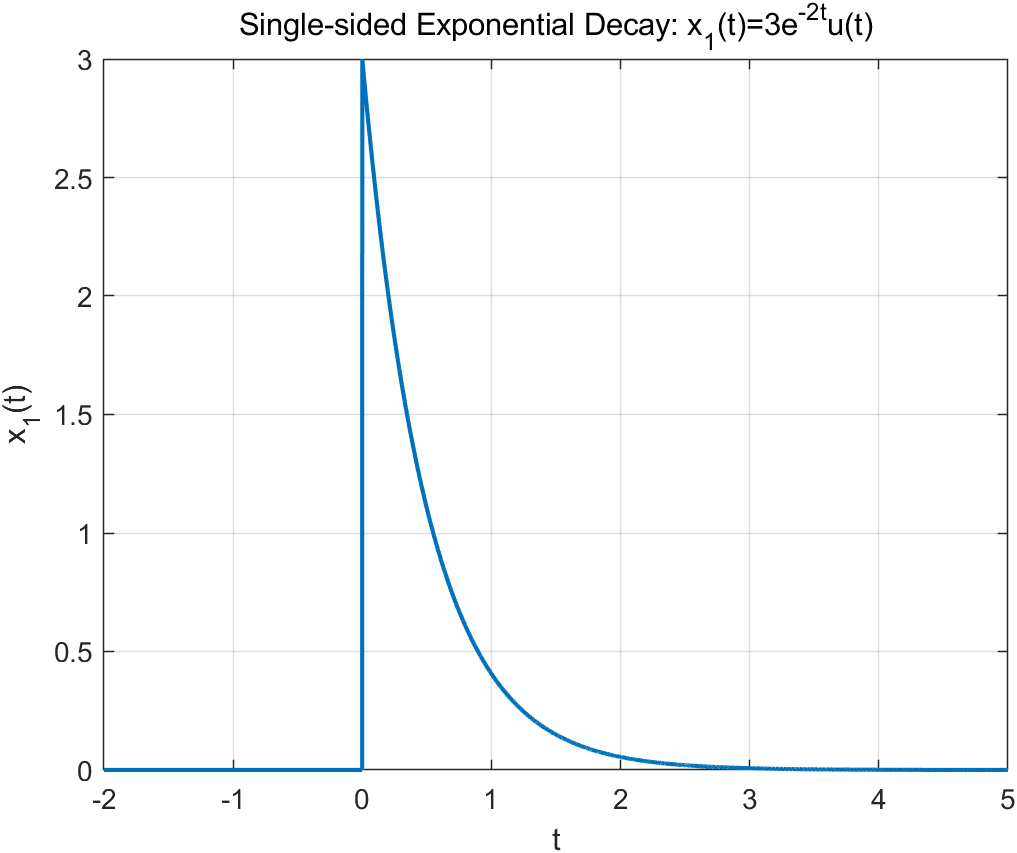
\includegraphics[width=\linewidth]{figures/Q1_1_fig1.png}
        \caption{Single-sided exponential decay.}
    \end{subfigure}
    \begin{subfigure}{0.48\textwidth}
        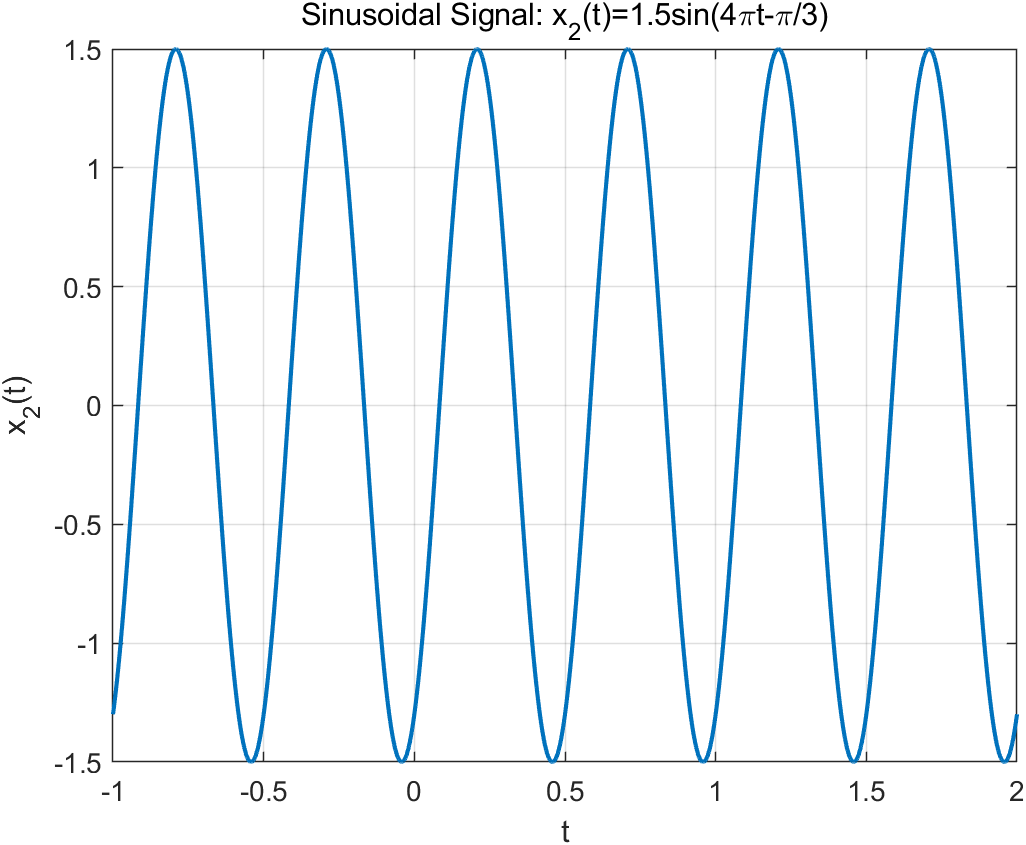
\includegraphics[width=\linewidth]{figures/Q1_1_fig2.png}
        \caption{Sinusoidal signal.}
    \end{subfigure}
    \begin{subfigure}{0.48\textwidth}
        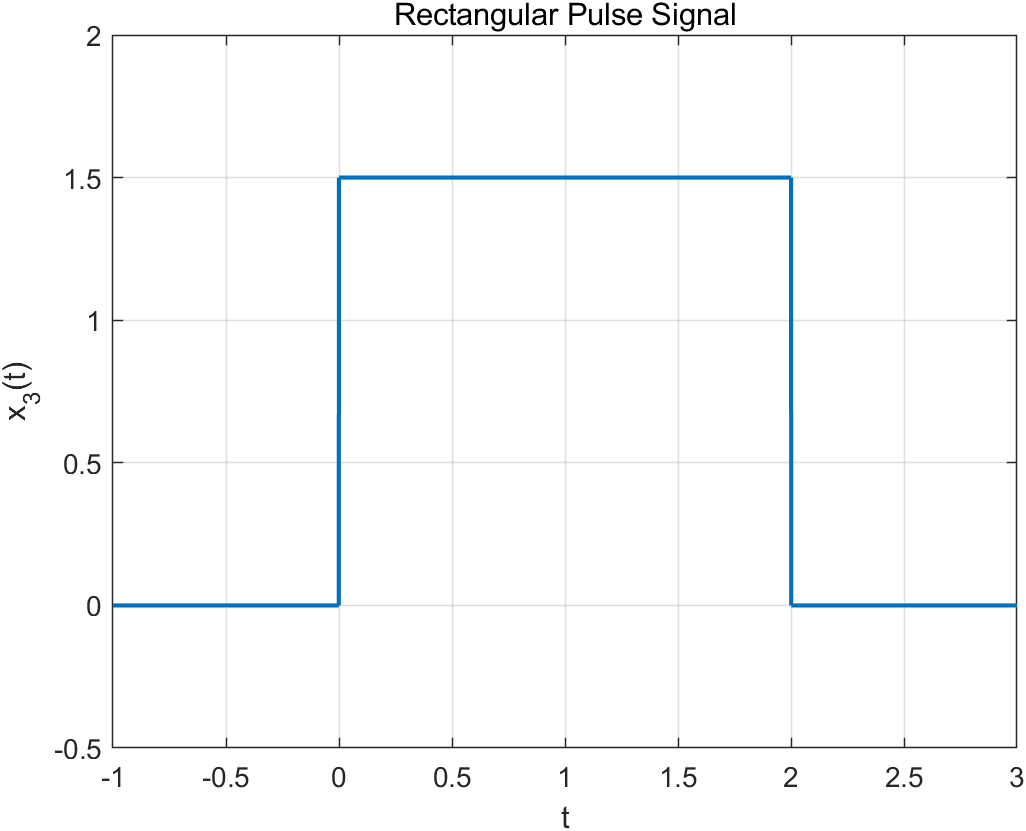
\includegraphics[width=\linewidth]{figures/Q1_1_fig3.png}
        \caption{Rectangular pulse.}
    \end{subfigure}
    \begin{subfigure}{0.48\textwidth}
        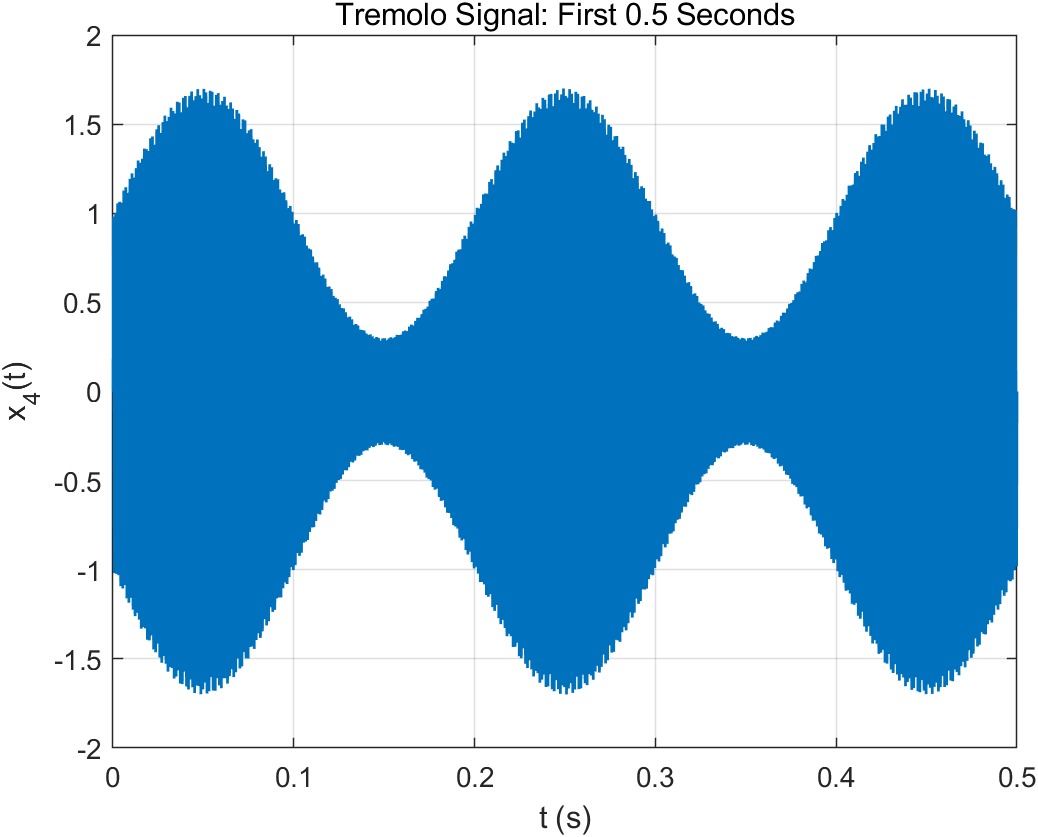
\includegraphics[width=\linewidth]{figures/Q1_1_fig4.png}
        \caption{Tremolo signal.}
    \end{subfigure}
    \caption{Experiment 1.1 generated continuous-time signals.}
\end{figure}

The exponential signal is zero before \(t=0\) and decays after the step activates it. The sinusoidal waveform has the expected amplitude and phase shift. The rectangular pulse is centred in the display using an adjusted axis range. The tremolo signal shows a high-frequency sinusoid whose amplitude envelope changes slowly at 5 Hz.

\section{Experiment 1.2: Basic Operations on Continuous-Time Signals}

\subsection{Problem Statement}
The given signal is
\[
f(t)=
\begin{cases}
t+1, & -1\leq t\leq 0,\\
1-t, & 0<t\leq 1,\\
0, & \text{otherwise}.
\end{cases}
\]
The task is to plot \(f(t)\), \(f(t-2)\), \(f(3t)\), \(f(-t)\), and \(f(-3t-2)\) over \(-3\leq t\leq 3\).

\subsection{Principle and Formula Explanation}
A time shift is obtained by replacing \(t\) with \(t-t_0\). A time scaling \(f(at)\) compresses the signal by a factor of \(|a|\) when \(|a|>1\). A negative argument produces time reversal. The composite signal \(f(-3t-2)\) combines reversal, compression, and shifting.

\subsection{Key MATLAB Code}
\begin{lstlisting}[style=matlabstyle]
t = -3:0.001:3;
f = (t+1).*(t>=-1 & t<=0) + ...
    (1-t).*(t>0 & t<=1);

t_shift = t - 2;
f_shift = (t_shift+1).*(t_shift>=-1 & t_shift<=0) + ...
          (1-t_shift).*(t_shift>0 & t_shift<=1);

t_mix = -3*t - 2;
f_mix = (t_mix+1).*(t_mix>=-1 & t_mix<=0) + ...
        (1-t_mix).*(t_mix>0 & t_mix<=1);
\end{lstlisting}

\subsection{Code Analysis}
The same piecewise definition is reused after substituting the transformed argument. This directly follows the mathematical definition of signal transformation and reduces implementation errors.

\subsection{Results and Interpretation}
\begin{figure}[H]
    \centering
    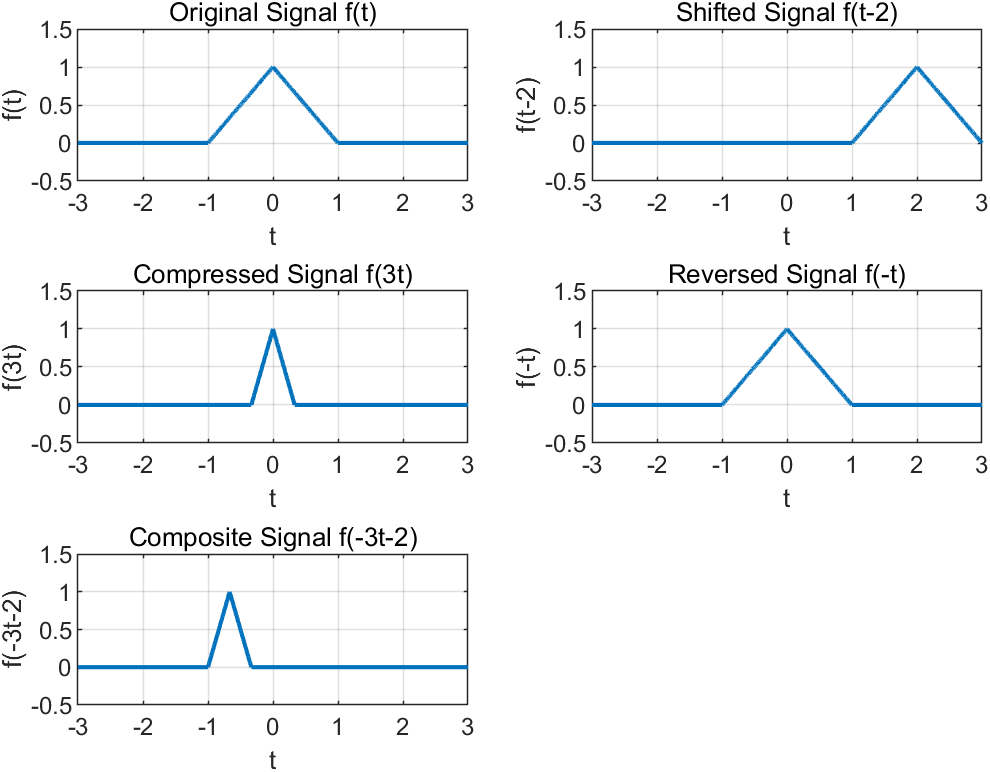
\includegraphics[width=0.9\textwidth]{figures/Q1_2_fig1.png}
    \caption{Original and transformed versions of \(f(t)\).}
\end{figure}

The plot confirms that \(f(t-2)\) shifts the signal two units to the right, \(f(3t)\) compresses it in time, and \(f(-t)\) mirrors it about the vertical axis. For \(f(-3t-2)\), the order of operations matters unless the same final algebraic argument is preserved. The relationship between \(f(3t)\) and \(f(t/3)\) is opposite in time scale: the former compresses by 3, while the latter expands by 3.

\section{Experiment 1.3: Time-Domain Analysis of a Continuous-Time LTI System}

\subsection{Problem Statement}
The LTI system is described by
\[
y''(t)+3y'(t)+2y(t)=x'(t)+2x(t),
\]
with input
\[
x(t)=e^{-2t}u(t).
\]
The tasks are to determine the transfer-function coefficients, plot the impulse response, and plot the zero-state response.

\subsection{Principle and Formula Explanation}
Taking the Laplace transform under zero initial conditions gives
\[
(s^2+3s+2)Y(s)=(s+2)X(s).
\]
Therefore,
\[
H(s)=\frac{Y(s)}{X(s)}=\frac{s+2}{s^2+3s+2}
=\frac{s+2}{(s+1)(s+2)}=\frac{1}{s+1}.
\]
The impulse response is the inverse Laplace transform:
\[
h(t)=e^{-t}u(t).
\]
The zero-state response is the convolution
\[
y_{zs}(t)=x(t)*h(t)=\int_0^t e^{-2\tau}e^{-(t-\tau)}\,d\tau
=e^{-t}-e^{-2t}.
\]

\subsection{Key MATLAB Code}
\begin{lstlisting}[style=matlabstyle]
num = [1 2];
den = [1 3 2];
t = 0:0.001:5;
x = exp(-2*t);

if exist('tf','file') && exist('impulse','file') && exist('lsim','file')
    sys = tf(num, den);
    [h, th] = impulse(sys, t);
    yzs = lsim(sys, x, t);
else
    th = t;
    h = exp(-t);
    yzs = exp(-t) - exp(-2*t);
end
\end{lstlisting}

\subsection{Code Analysis}
The coefficient vectors are \(\texttt{num=[1 2]}\) and \(\texttt{den=[1 3 2]}\). The implementation calls the required Control System Toolbox functions when available. Since the verified local environment does not include that toolbox, an analytical fallback is used to preserve the same mathematical result.

\subsection{Results and Interpretation}
\begin{figure}[H]
    \centering
    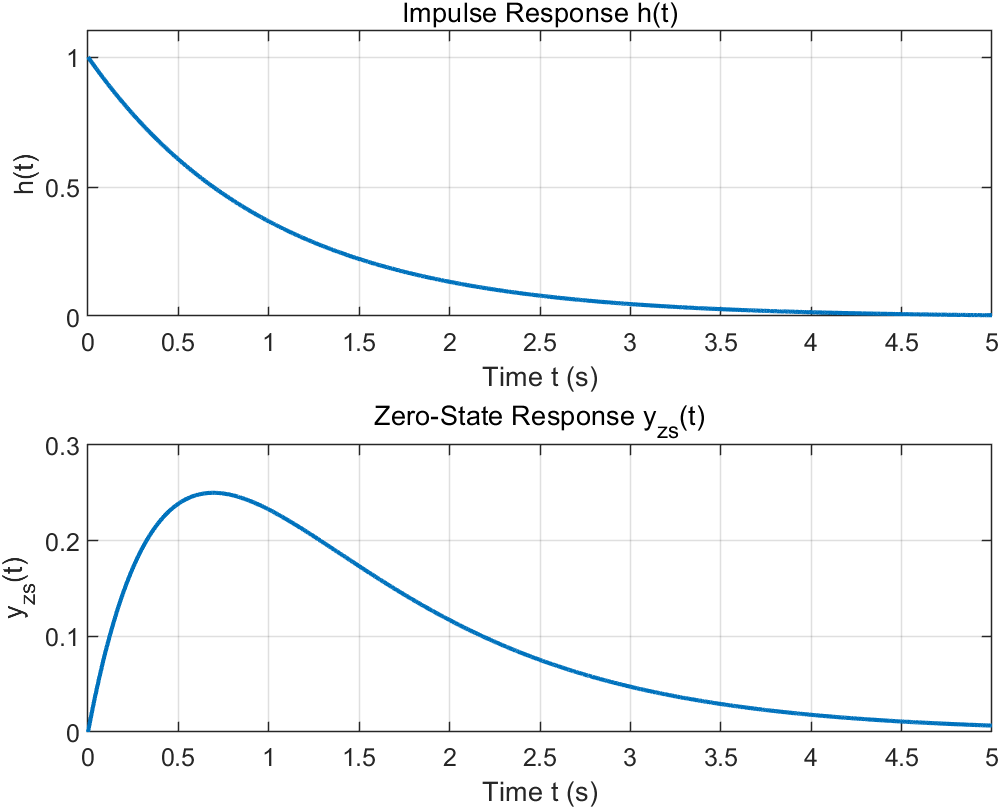
\includegraphics[width=0.8\textwidth]{figures/Q1_3_fig1.png}
    \caption{Impulse response and zero-state response.}
\end{figure}

The impulse response decays exponentially, indicating a stable first-order effective system. The zero-state response initially rises from zero and then decays because the input and impulse response are both causal exponentials.

\section{Experiment 1.4: Numerical Convolution of Continuous-Time Signals}

\subsection{Problem Statement}
The signals are
\[
f_1(t)=
\begin{cases}
1.5, & -1\leq t\leq 1,\\
0, & \text{otherwise},
\end{cases}
\quad
f_2(t)=
\begin{cases}
2, & -1\leq t\leq 1,\\
0, & \text{otherwise}.
\end{cases}
\]
The task is to compute \(y(t)=f_1(t)*f_2(t)\) numerically using different sampling intervals and evaluate the error relative to a fine reference result.

\subsection{Principle and Formula Explanation}
Continuous convolution is defined as
\[
y(t)=\int_{-\infty}^{\infty}f_1(\tau)f_2(t-\tau)\,d\tau.
\]
The discrete approximation with sampling interval \(p\) is
\[
y[n]\approx p\sum_k f_1[k]f_2[n-k].
\]
The factor \(p\) is required because MATLAB's \texttt{conv} computes a summation, whereas the continuous convolution is an integral.

\subsection{Key MATLAB Code}
\begin{lstlisting}[style=matlabstyle]
p_values = [0.2 0.1 0.05 0.02];
for i = 1:length(p_values)
    p = p_values(i);
    t = -2:p:2;
    f1 = 1.5 * double(t >= -1 & t <= 1);
    f2 = 2 * double(t >= -1 & t <= 1);
    y = conv(f1, f2) * p;
    ty = (min(t)+min(t)):p:(max(t)+max(t));
end
\end{lstlisting}

\subsection{Code Analysis}
The output time vector spans the sum of the input supports. Interpolation is used to compare coarser results with the fine reference grid at \(p=0.001\).

\subsection{Results, Numerical Analysis, and Interpretation}
\begin{figure}[H]
    \centering
    \begin{subfigure}{0.48\textwidth}
        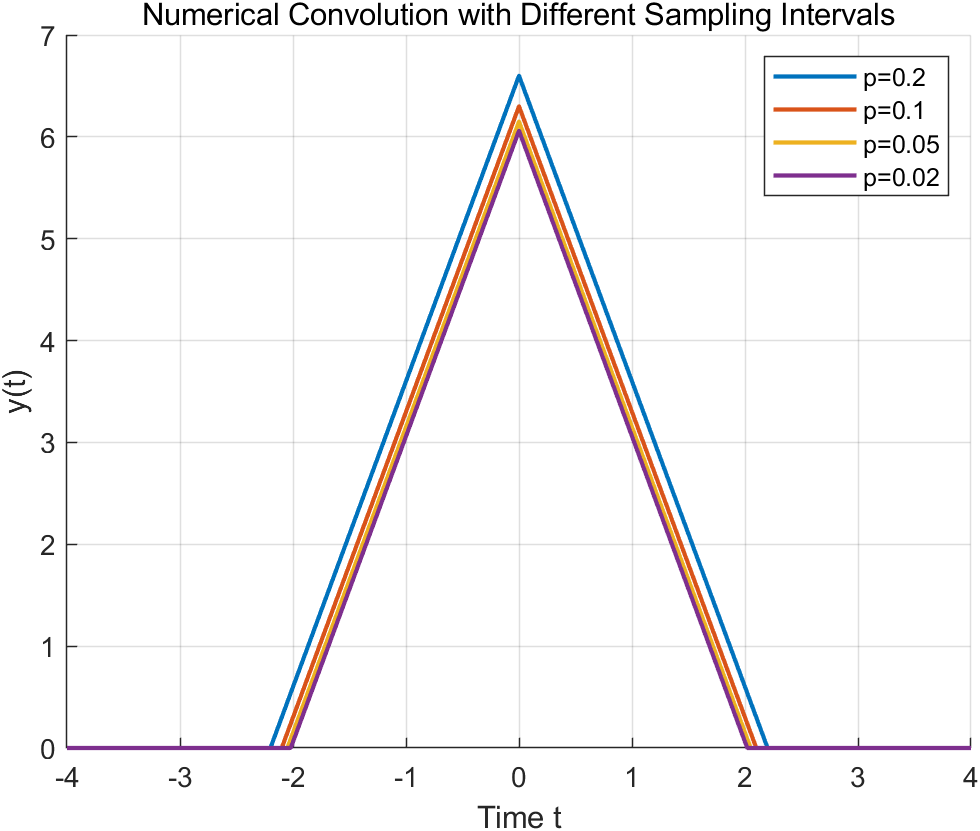
\includegraphics[width=\linewidth]{figures/Q1_4_fig1.png}
        \caption{Results for different sampling intervals.}
    \end{subfigure}
    \begin{subfigure}{0.48\textwidth}
        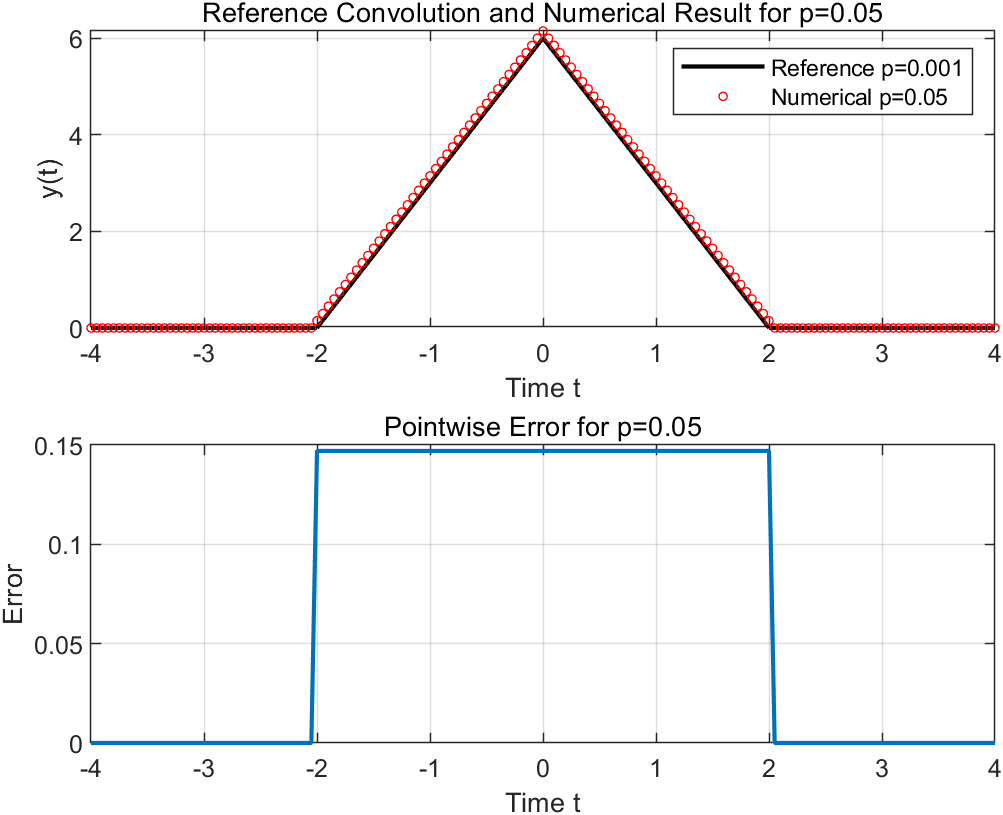
\includegraphics[width=\linewidth]{figures/Q1_4_fig2.png}
        \caption{Reference comparison and pointwise error.}
    \end{subfigure}
    \caption{Numerical convolution results.}
\end{figure}

\begin{table}[H]
\centering
\caption{Numerical convolution error relative to \(p=0.001\).}
\begin{tabular}{ccc}
\toprule
Sampling interval \(p\) & MSE & Maximum absolute error\\
\midrule
0.200 & 0.184181 & 0.597000\\
0.100 & 0.044849 & 0.297000\\
0.050 & 0.010897 & 0.147000\\
0.020 & 0.001630 & 0.057000\\
\bottomrule
\end{tabular}
\end{table}

As \(p\) decreases, the approximation becomes smoother and closer to the reference triangular convolution. If \(p\) is too large, the rectangular pulses are poorly sampled, causing inaccurate overlap estimation and larger numerical error.

\section{Experiment 2.1: Fourier Series Analysis of Periodic Rectangular Pulses}

\subsection{Problem Statement}
For periodic rectangular pulses with period \(T=8\) and widths \(\tau=4,2,1\), compute and plot the magnitude spectra \(|c_k|\) for \(k=-20,\ldots,20\).

\subsection{Principle and Formula Explanation}
The exponential Fourier series coefficients are
\[
c_k=\frac{\tau}{T}\operatorname{sinc}\left(\frac{k\tau}{T}\right),
\quad
\operatorname{sinc}(x)=\frac{\sin(\pi x)}{\pi x}.
\]
The DC component is
\[
c_0=\frac{\tau}{T}.
\]

\subsection{Key MATLAB Code}
\begin{lstlisting}[style=matlabstyle]
T = 8;
tau_values = [4 2 1];
k = -20:20;
for i = 1:length(tau_values)
    tau = tau_values(i);
    ck = (tau/T) * sinc(k*tau/T);
    stem(k, abs(ck), 'filled');
end
\end{lstlisting}

\subsection{Code Analysis}
MATLAB's normalized \texttt{sinc} function matches the coursework definition. Each value of \(\tau\) changes the coefficient envelope but not the spacing of the integer harmonic index \(k\).

\subsection{Results and Interpretation}
\begin{figure}[H]
    \centering
    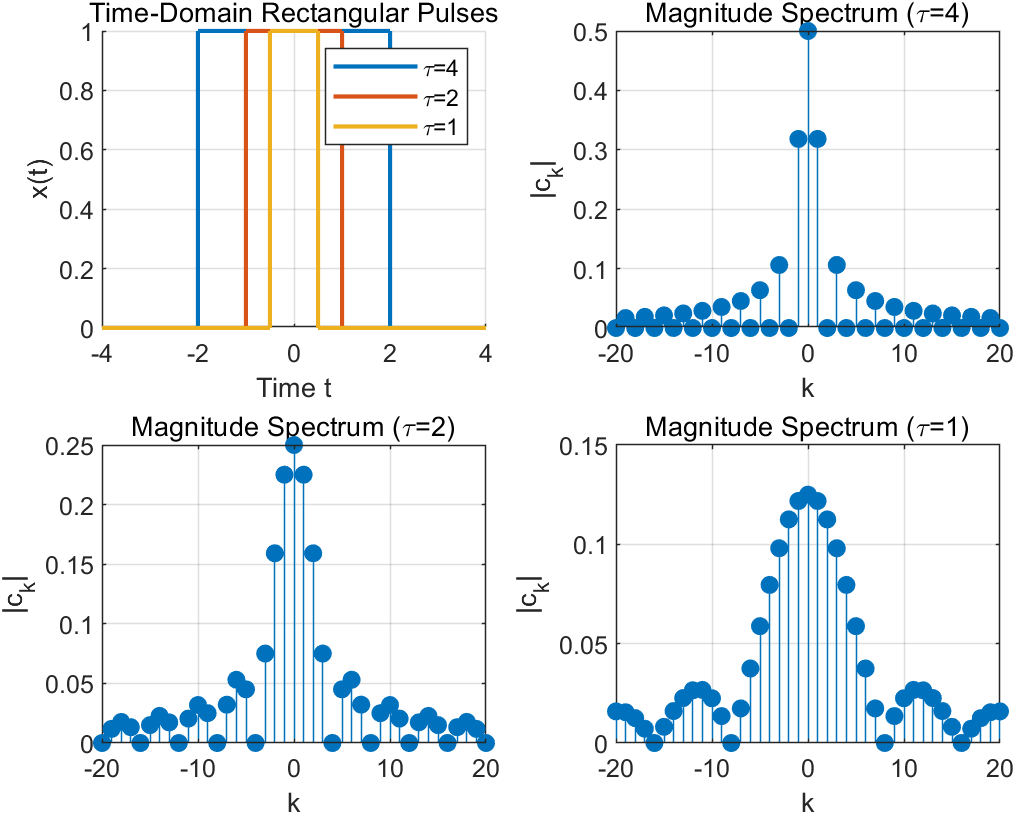
\includegraphics[width=0.85\textwidth]{figures/Q2_1_fig1.png}
    \caption{Time-domain rectangular pulses and their Fourier series magnitude spectra.}
\end{figure}

When the pulse width decreases, the main lobe in the frequency-domain envelope becomes wider. The spacing between spectral lines is controlled by the period \(T\), so it remains unchanged. The DC component decreases from \(4/8\) to \(2/8\) and \(1/8\), consistent with the duty cycle.

\section{Experiment 2.2: Frequency-Domain Analysis of a Continuous-Time LTI System}

\subsection{Problem Statement}
The system has frequency response
\[
H(j\omega)=\frac{1}{(j\omega)^2+2j\omega+5}.
\]
The input is
\[
x(t)=3\cos(2t)+2\cos(15t).
\]
The task is to evaluate the magnitude and phase response at \(\omega=2\) and \(\omega=15\), then construct and plot the output.

\subsection{Principle and Formula Explanation}
For an LTI system, a sinusoid at frequency \(\omega_0\) remains a sinusoid at the same frequency, but its amplitude and phase are modified:
\[
A\cos(\omega_0t)\rightarrow A|H(j\omega_0)|\cos(\omega_0t+\angle H(j\omega_0)).
\]
Thus,
\[
y(t)=3|H(j2)|\cos(2t+\angle H(j2))
+2|H(j15)|\cos(15t+\angle H(j15)).
\]

\subsection{Key MATLAB Code}
\begin{lstlisting}[style=matlabstyle]
H = @(w) 1 ./ ((1i*w).^2 + 2*1i*w + 5);
H2 = H(2); H15 = H(15);
y = 3*abs(H2)*cos(2*t + angle(H2)) + ...
    2*abs(H15)*cos(15*t + angle(H15));
\end{lstlisting}

\subsection{Results, Numerical Values, and Interpretation}
\begin{figure}[H]
    \centering
    \begin{subfigure}{0.48\textwidth}
        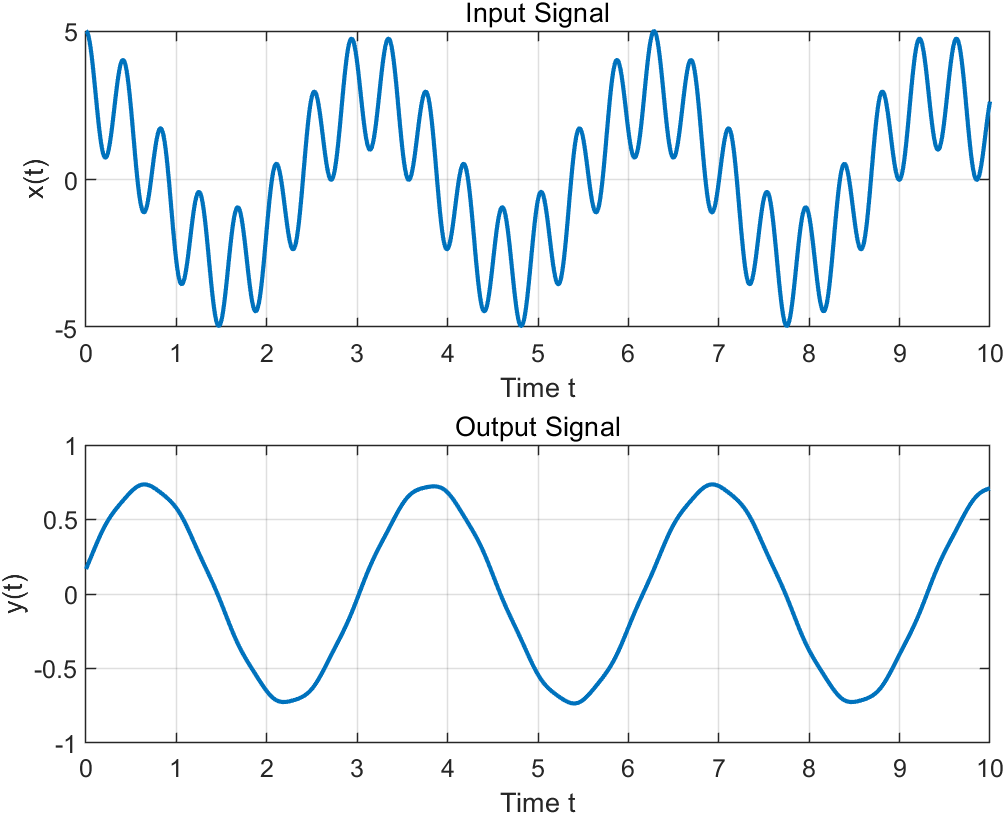
\includegraphics[width=\linewidth]{figures/Q2_2_fig1.png}
        \caption{Input and output waveforms.}
    \end{subfigure}
    \begin{subfigure}{0.48\textwidth}
        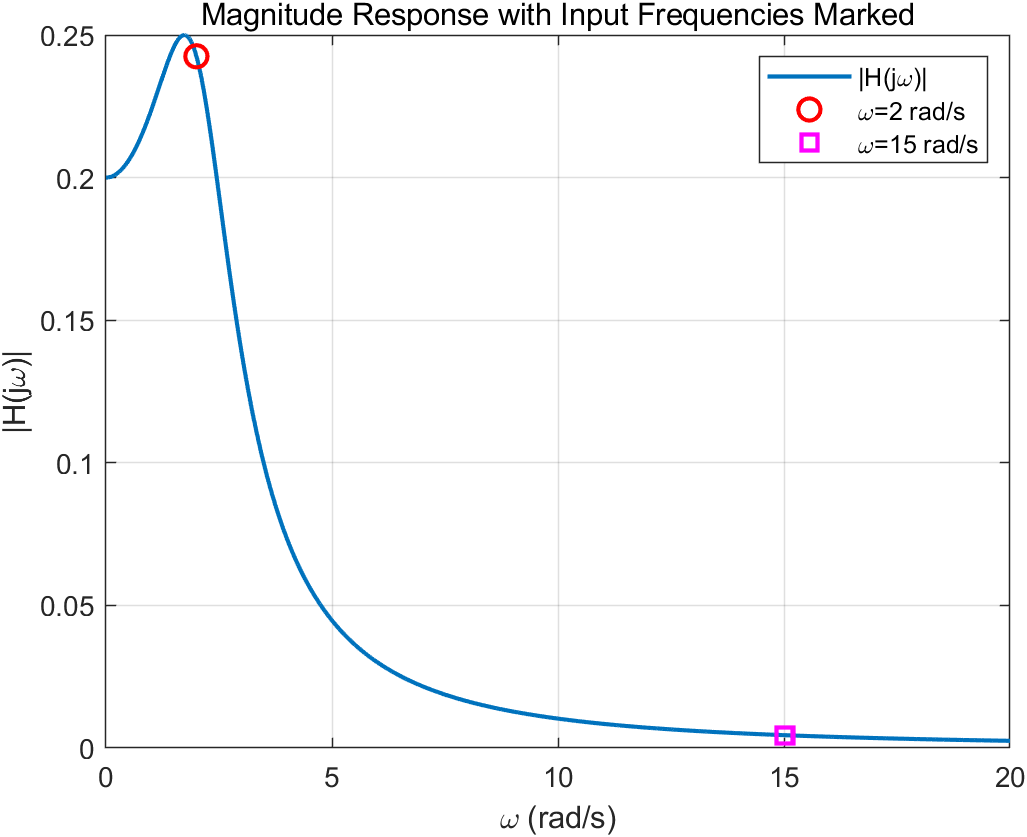
\includegraphics[width=\linewidth]{figures/Q2_2_fig2.png}
        \caption{Magnitude response with marked input frequencies.}
    \end{subfigure}
    \caption{Frequency-domain response analysis.}
\end{figure}

\begin{table}[H]
\centering
\caption{Frequency response values.}
\begin{tabular}{ccc}
\toprule
Frequency & Magnitude & Phase\\
\midrule
\(\omega=2\) & 0.2425 & \(-1.3258\) rad\\
\(\omega=15\) & 0.0045 & \(-3.0061\) rad\\
\bottomrule
\end{tabular}
\end{table}

The component at \(15\) rad/s is strongly attenuated compared with the component at \(2\) rad/s. Therefore, the system behaves approximately as a low-pass filter.

\section{Experiment 3.1: RLC Second-Order Low-Pass Filter}

\subsection{Problem Statement}
For an RLC low-pass filter with \(L=0.6\) H, \(C=0.2\) F, and \(R=2\,\Omega\),
\[
H(s)=\frac{1}{LCs^2+RCs+1}.
\]
The tasks are to plot magnitude and phase responses using \texttt{freqs} and compute the zero-state response to
\[
x(t)=\sin(t)+\sin(20t).
\]

\subsection{Principle and Formula Explanation}
With the given component values,
\[
H(s)=\frac{1}{0.12s^2+0.4s+1}.
\]
Low-frequency components pass with relatively high gain, while high-frequency components are attenuated because the \(s^2\) term dominates the denominator at high \(\omega\).

\subsection{Key MATLAB Code}
\begin{lstlisting}[style=matlabstyle]
L = 0.6; C = 0.2; R = 2;
num = [1];
den = [L*C R*C 1];
w = 0:0.01:20;
H = freqs(num, den, w);
\end{lstlisting}

\subsection{Code Analysis}
The \texttt{freqs} function evaluates the analog frequency response. If \texttt{lsim} is unavailable, the equivalent differential equation
\[
0.12y''(t)+0.4y'(t)+y(t)=x(t)
\]
is solved numerically under zero initial conditions.

\subsection{Results and Interpretation}
\begin{figure}[H]
    \centering
    \begin{subfigure}{0.48\textwidth}
        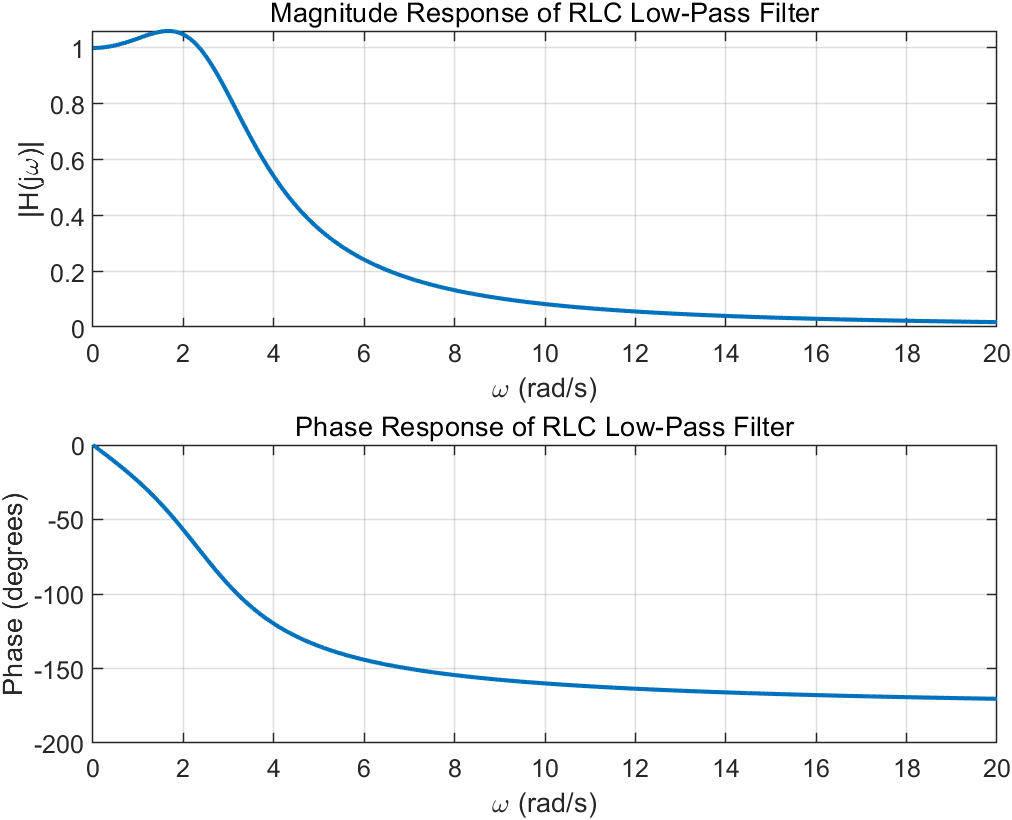
\includegraphics[width=\linewidth]{figures/Q3_1_fig1.png}
        \caption{Magnitude and phase response.}
    \end{subfigure}
    \begin{subfigure}{0.48\textwidth}
        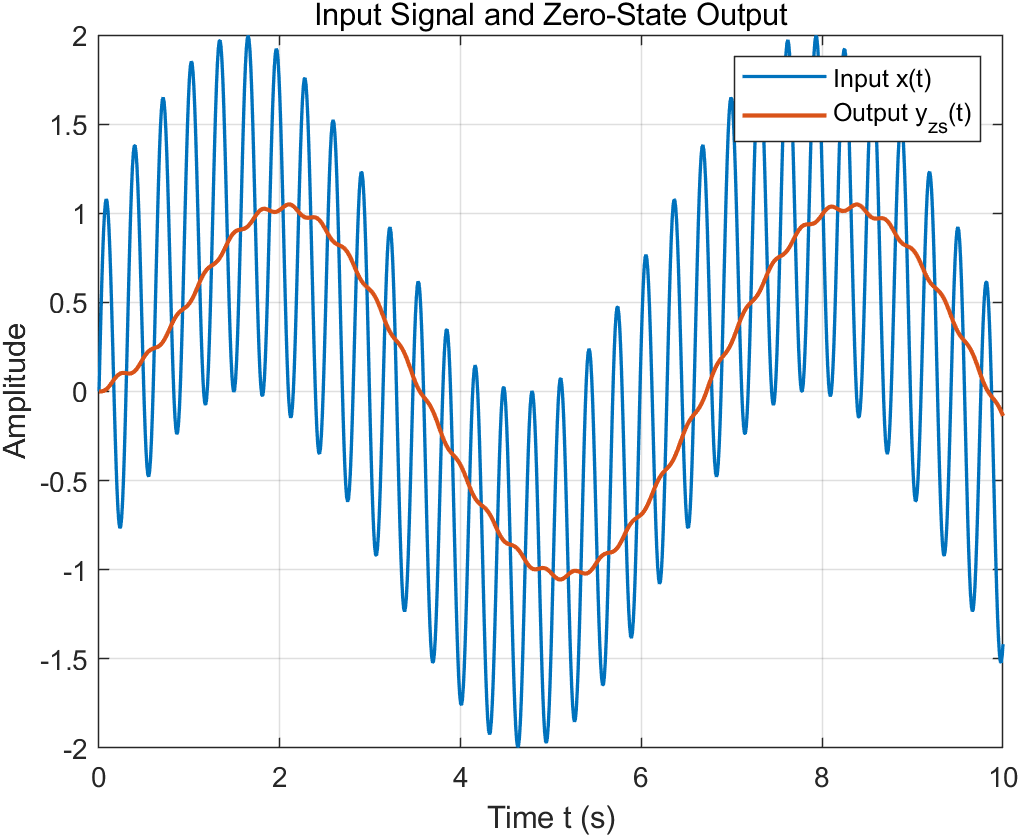
\includegraphics[width=\linewidth]{figures/Q3_1_fig2.png}
        \caption{Input and zero-state output.}
    \end{subfigure}
    \caption{RLC low-pass filter analysis.}
\end{figure}

The estimated \(-3\) dB cutoff frequency is approximately \(3.40\) rad/s. Therefore, the \(\sin(20t)\) component is attenuated much more than \(\sin(t)\). Increasing \(R\) would increase damping, reduce resonance, and smooth the transition of the response.

\section{Experiment 3.2: AM Modulation, Coherent Demodulation, and Low-Pass Filtering}

\subsection{Problem Statement}
The baseband signal and carrier are
\[
g(t)=4\cos(8t)+3\cos(16t),\quad c(t)=\cos(120t).
\]
The modulated and demodulated signals are
\[
f(t)=g(t)c(t),\quad g_0(t)=f(t)c(t).
\]
An ideal low-pass filter with cutoff \(|\omega|<25\) is used to recover \(g_1(t)\).

\subsection{Principle and Formula Explanation}
Using the identity
\[
\cos a\cos b=\frac{1}{2}\left[\cos(a+b)+\cos(a-b)\right],
\]
the modulation process shifts baseband components to \(120\pm 8\) and \(120\pm 16\) rad/s. Coherent demodulation gives
\[
g_0(t)=g(t)\cos^2(120t)
=\frac{1}{2}g(t)+\frac{1}{2}g(t)\cos(240t).
\]
After low-pass filtering, the high-frequency term is removed:
\[
g_1(t)\approx \frac{1}{2}g(t).
\]
Therefore, amplitude restoration requires multiplication by 2.

\subsection{Key MATLAB Code}
\begin{lstlisting}[style=matlabstyle]
g = 4*cos(8*t) + 3*cos(16*t);
c = cos(120*t);
f = g .* c;
g0 = f .* c;

G0_shift = fftshift(fft(g0));
H = double(abs(omega) < 25);
G1_shift = G0_shift .* H;
g1 = real(ifft(ifftshift(G1_shift)));
g1_restored = 2*g1;
\end{lstlisting}

\subsection{Code Analysis}
FFT and \texttt{fftshift} are used to implement an ideal frequency-domain low-pass filter. The cutoff keeps the baseband frequencies at 8 and 16 rad/s and rejects the components near 240 rad/s.

\subsection{Results, Numerical Analysis, and Interpretation}
\begin{figure}[H]
    \centering
    \begin{subfigure}{0.48\textwidth}
        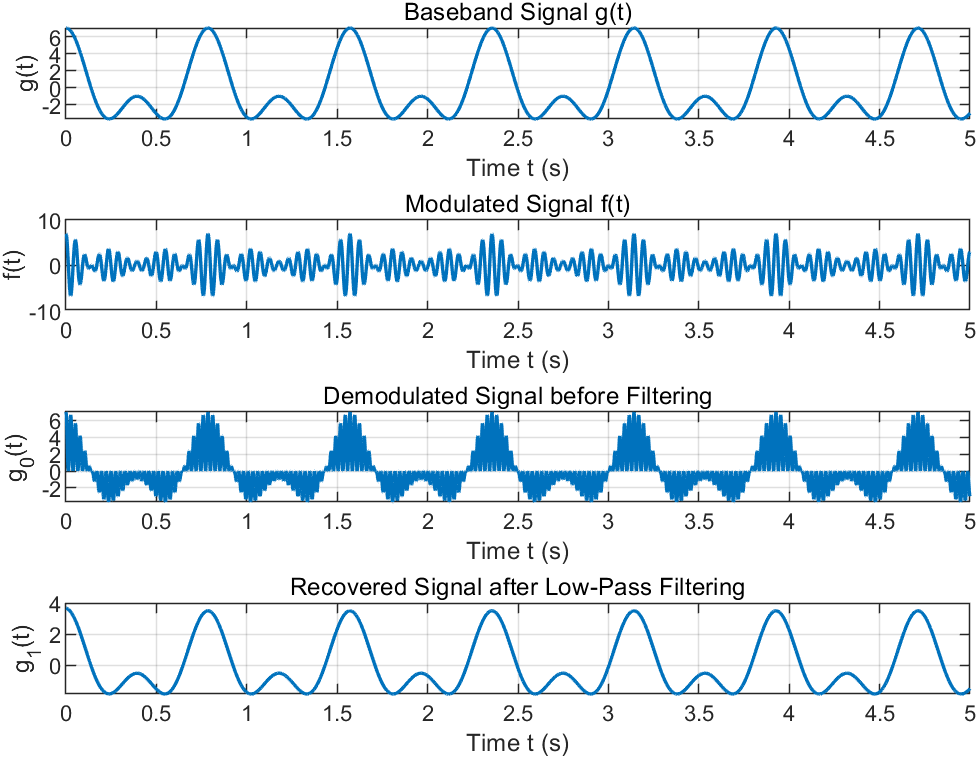
\includegraphics[width=\linewidth]{figures/Q3_2_fig1.png}
        \caption{Time-domain signals.}
    \end{subfigure}
    \begin{subfigure}{0.48\textwidth}
        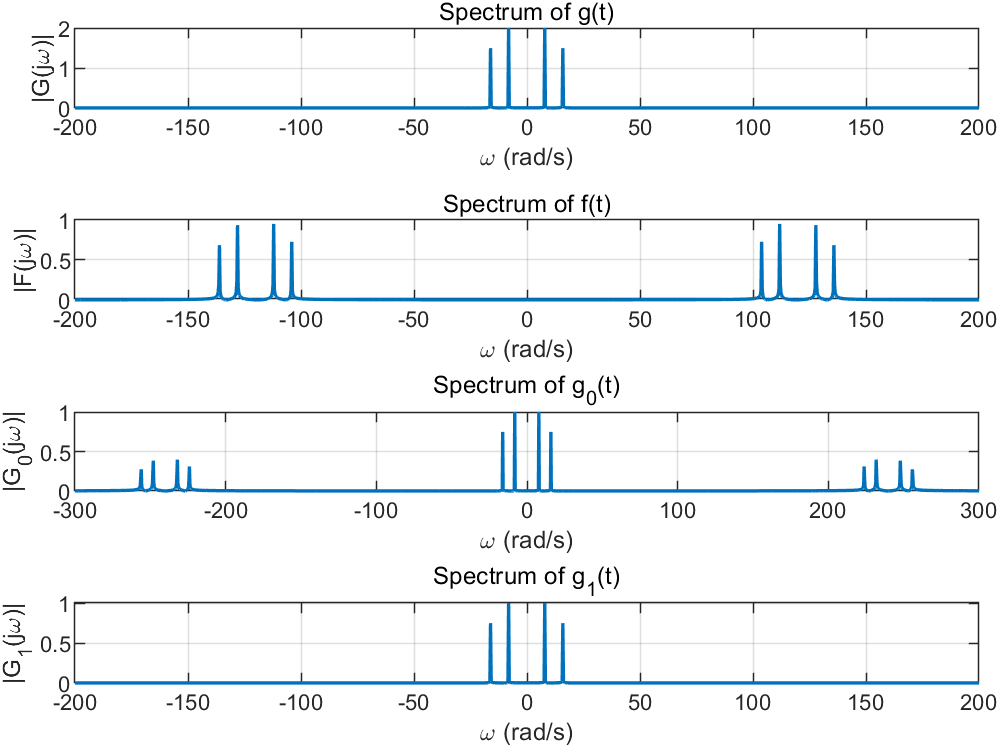
\includegraphics[width=\linewidth]{figures/Q3_2_fig2.png}
        \caption{Frequency spectra.}
    \end{subfigure}
    \begin{subfigure}{0.72\textwidth}
        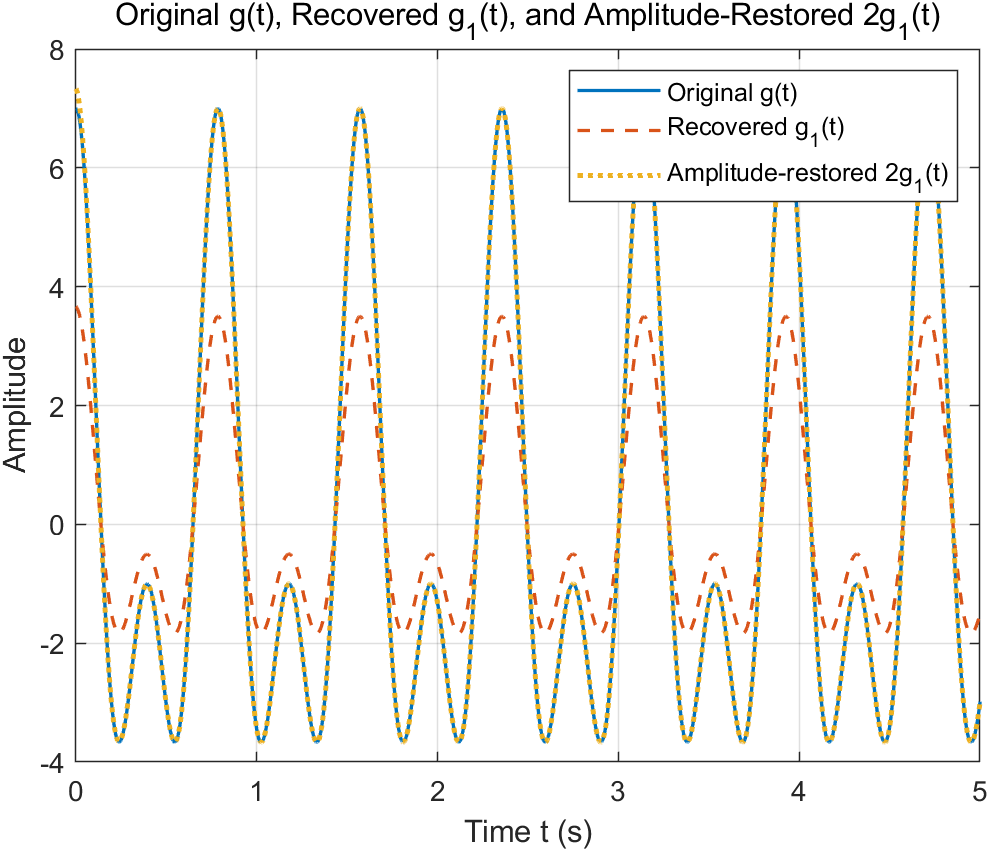
\includegraphics[width=\linewidth]{figures/Q3_2_fig3.png}
        \caption{Amplitude restoration comparison.}
    \end{subfigure}
    \caption{AM modulation and coherent demodulation results.}
\end{figure}

The verified mean-squared error between \(g(t)\) and \(g_1(t)\) is 3.124869. After amplitude restoration, the MSE between \(g(t)\) and \(2g_1(t)\) decreases to 0.000310. This confirms that the recovered waveform shape is correct, while the main difference is the expected factor of one half from coherent demodulation.

\section{Experiment 4.1: Geometric Evaluation of Frequency Response from Pole-Zero Plot}

\subsection{Problem Statement}
The system has poles
\[
p_1=-80,\quad p_2=-120
\]
and a double zero at the origin:
\[
z_1=z_2=0.
\]
For \(f=0\) to \(1000\) Hz, compute
\[
|H(j\omega)|=
\frac{|j\omega-z_1||j\omega-z_2|}
{|j\omega-p_1||j\omega-p_2|},
\quad \omega=2\pi f.
\]
The result must be compared with MATLAB's \texttt{freqs} function.

\subsection{Principle and Formula Explanation}
The geometric method evaluates frequency response by measuring vector lengths in the \(s\)-plane from each zero and pole to the point \(j\omega\). Zeros contribute to the numerator and poles contribute to the denominator. A double zero at the origin makes low-frequency gain small, which is characteristic of high-pass behaviour.

\subsection{Key MATLAB Code}
\begin{lstlisting}[style=matlabstyle]
f = 0:1:1000;
omega = 2*pi*f;
H_geo = (abs(1i*omega-z1).*abs(1i*omega-z2)) ./ ...
        (abs(1i*omega-p1).*abs(1i*omega-p2));

num_tf = [1 0 0];
den_tf = conv([1 80], [1 120]);
H_freqs = freqs(num_tf, den_tf, omega);
\end{lstlisting}

\subsection{Results and Interpretation}
\begin{figure}[H]
    \centering
    \begin{subfigure}{0.48\textwidth}
        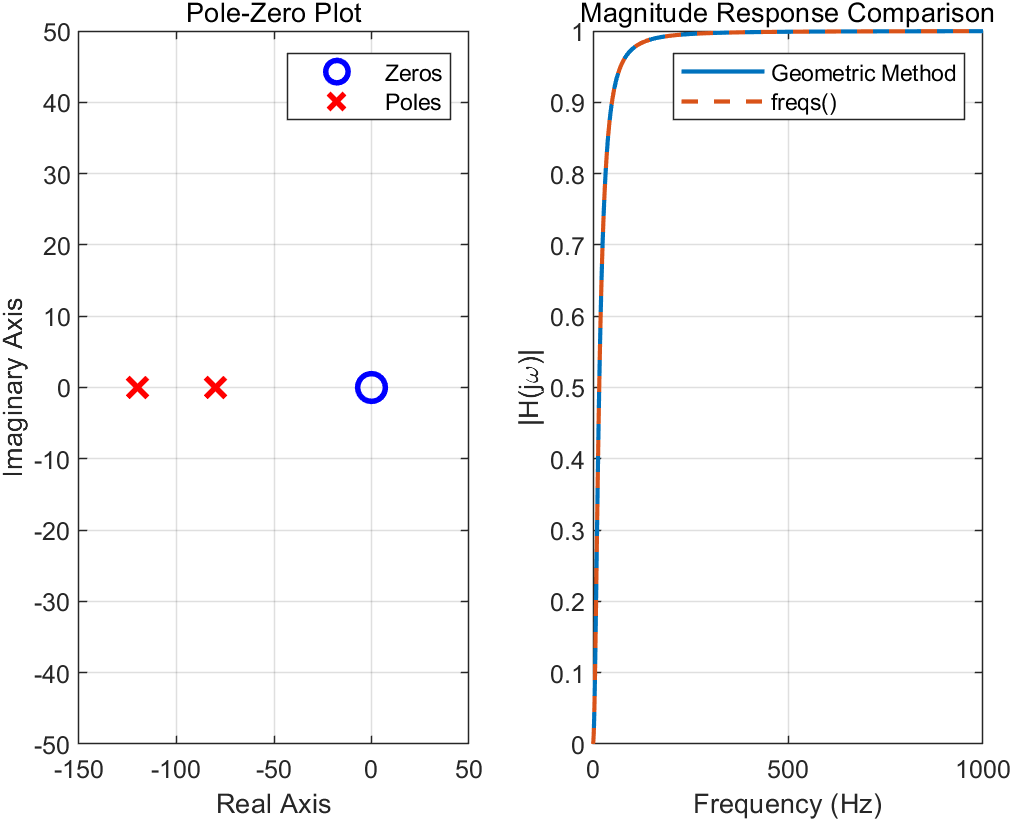
\includegraphics[width=\linewidth]{figures/Q4_1_fig1.png}
        \caption{Pole-zero plot and magnitude response comparison.}
    \end{subfigure}
    \begin{subfigure}{0.48\textwidth}
        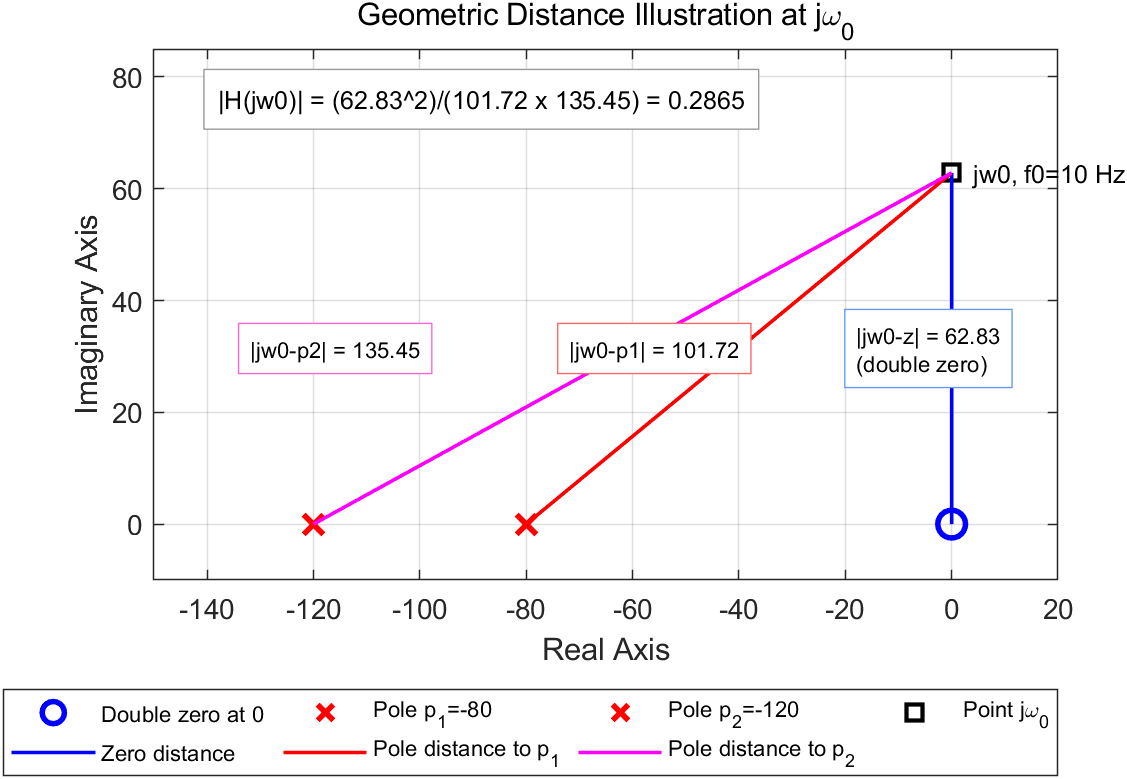
\includegraphics[width=\linewidth]{figures/Q4_1_fig2.png}
        \caption{Geometric distance illustration.}
    \end{subfigure}
    \caption{Geometric frequency-response evaluation.}
\end{figure}

The geometric result and the \texttt{freqs} result overlap, verifying the computation. The supplementary illustration at \(f_0=10\) Hz shows the distance vectors directly. At that point,
\[
|H(j\omega_0)|=
\frac{62.83^2}{101.72\times 135.45}=0.2865.
\]
The response rises with frequency because the double zero at the origin suppresses low-frequency gain.

\section{Experiment 4.2: Pole-Zero Map and Stability}

\subsection{Problem Statement}
For the system
\[
H(s)=\frac{s^2+4s+3}{s^3+s^2+7s+2},
\]
plot the pole-zero map and determine whether the system is stable.

\subsection{Principle and Formula Explanation}
The zeros are roots of the numerator and the poles are roots of the denominator. A continuous-time LTI system is BIBO stable if all poles lie in the open left half-plane:
\[
\operatorname{Re}(p_i)<0,\quad \forall i.
\]
Pole locations also indicate damping and oscillatory characteristics. For a complex pole \(p=\sigma+j\omega_d\),
\[
\omega_n=|p|,\quad \zeta=-\frac{\sigma}{\omega_n}.
\]

\subsection{Key MATLAB Code}
\begin{lstlisting}[style=matlabstyle]
num = [1 4 3];
den = [1 1 7 2];
z = roots(num);
p = roots(den);

if all(real(p) < 0)
    disp('Stability: stable because all poles lie in the left half-plane.');
end
\end{lstlisting}

\subsection{Results, Numerical Analysis, and Interpretation}
\begin{figure}[H]
    \centering
    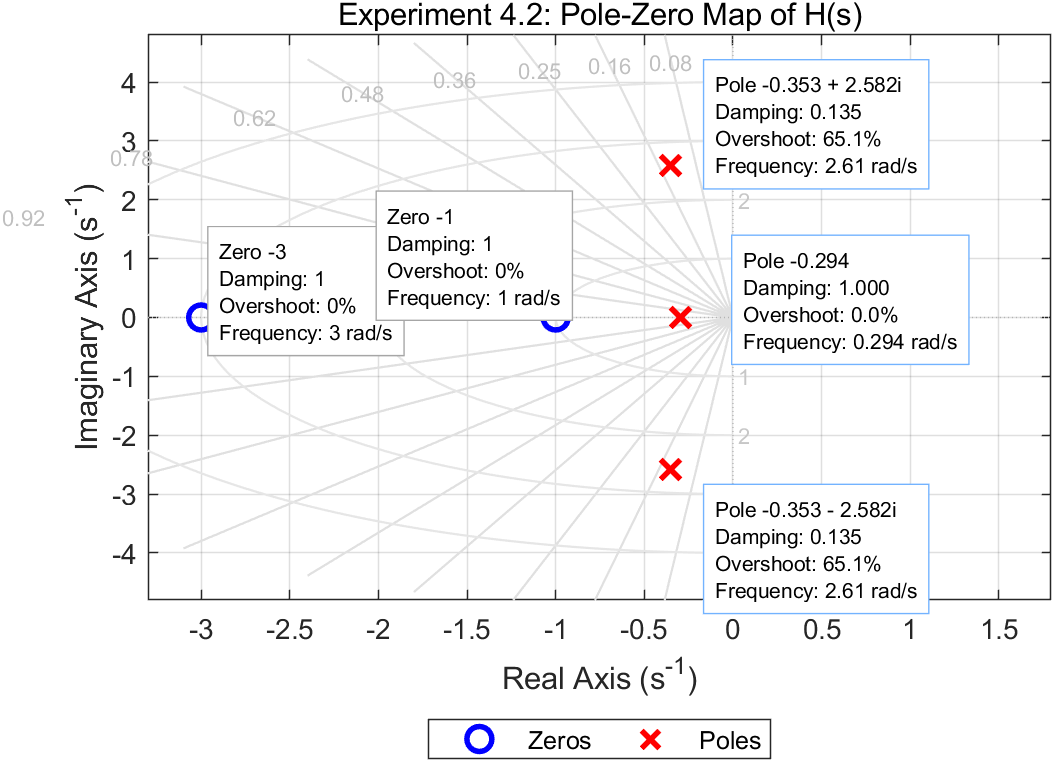
\includegraphics[width=0.85\textwidth]{figures/Q4_2_fig1.png}
    \caption{Enhanced pole-zero map with damping-ratio grid and annotations.}
\end{figure}

The zeros are \(-3\) and \(-1\). The poles are approximately
\[
-0.3528\pm j2.5822,\quad -0.2945.
\]
All poles have negative real parts; therefore, the system is stable. The complex pole pair has damping ratio approximately \(0.1354\) and natural frequency approximately \(2.6062\) rad/s, indicating an underdamped mode.

\section{Discussion and Conclusion}
The experiments collectively verify several core principles in continuous-time signals and systems. First, basic signals can be represented accurately in MATLAB using vectorized time grids and logical masks. Second, time shifting, scaling, and reversal can be implemented by substituting the transformed argument into the original signal definition. Third, LTI system responses are governed by the transfer function: the impulse response is the inverse transform of \(H(s)\), while the zero-state response is the convolution of the input and impulse response.

Numerical convolution results show that the sampling interval strongly affects approximation accuracy. The MSE decreases from 0.184181 at \(p=0.2\) to 0.001630 at \(p=0.02\), confirming that smaller sampling intervals better approximate the continuous convolution integral. Fourier series analysis shows the inverse relationship between time-domain pulse width and frequency-domain bandwidth: narrower pulses require wider spectral support. Frequency-domain LTI analysis confirms that sinusoidal inputs retain their frequencies while their amplitudes and phases are modified by \(H(j\omega)\).

The RLC circuit behaves as a low-pass filter with an estimated cutoff near \(3.40\) rad/s, attenuating the \(20\) rad/s component more strongly than the \(1\) rad/s component. The AM experiment confirms frequency translation during modulation and demonstrates that coherent demodulation followed by ideal low-pass filtering recovers a half-amplitude baseband signal. Multiplication by 2 restores the amplitude, reducing the MSE from 3.124869 to 0.000310. Finally, pole-zero analysis demonstrates both geometric frequency-response evaluation and stability assessment. The Experiment 4.1 geometric method agrees with \texttt{freqs}, and the Experiment 4.2 pole-zero map confirms stability because all poles are in the left half-plane.

Overall, the MATLAB simulations and analytical calculations are mutually consistent. The generated figures and numerical results support the theoretical expectations for each experiment and provide a complete verification of the coursework requirements.

\end{document}
